\documentclass[../book.tex]{subfiles}
\graphicspath{{\subfix{../images/}}}

\begin{document}
\chapter{Linear Functions and Relations}
\begin{introduction}[Contents]
\item Linear Functions
\item Inverses of Linear Functions
\item Piece-wise Linear Functions
\end{introduction}
\noindent Linear functions, other than constant functions $y(x)=c$ ($c\in\mathbb{R}$), are the most basic functions one can possible have.  This fact makes these functions fundamental when it comes to learning algebra and applying it in the real world.  All (univariate) linear functions can be put in the form $y(x)=mx+b$ where $m$ and $b$ are real numbers ($m\neq 0$ as this would result in a constant function).  One essential property which makes these functions so useful is that the \textit{rate of change} or \textit{slope} of the function is constant at every point; visually, this means the graph of the function does not curve.  

One common application which you, the reader, have most likely used without realizing it is unit conversion.  For example, when converting between inches and feet, it is understood that every $12$ inches in some given length is equivalent to 1 foot; this can be put into a linear relationship given by $f(i)=\dfrac{i}{12}$ where $f(i)$ represents the number of feet given a number of inches, and $i$ is the number of inches.  This relationship is based on the idea that $12$ inches will always equal to one foot, taking advantage of the property of a constant slope mentioned earlier seen in all linear functions.

This will be one of the shortest chapter in this text.  This entire chapter should serve as a review, but we included it to provide a comprehensive Algebra book.  Please read this chapter just like any other to make sure you didn't forget any information.
\section{Linear Functions}
\noindent Before we begin this section, it should be noted that most (if not all) of the material should be review from Algebra 1 and 2.

As previously stated in the introduction, all linear functions can be put into the form $y(x)=mx+b$, this is arguably the most common form, generally referred to as \textit{slope-intercept} form.  Indicative of the name, this form contains two pieces of information: the slope and y-intercept of the function.

Given two points with coordinates $(x_1,y_1)$ and $(x_2,y_2)$, the slope can be calculated by: $$m=\dfrac{\text{"rise"}}{\text{"run"}}=\dfrac{y_2-y_1}{x_2-x_1}=\dfrac{\Delta y}{\Delta x}.$$
\begin{note}
This is something that should already be memorized!  If not, commit it to memory as we will use this frequently for the rest of the chapter and in future chapters.
\end{note}
One of the downsides to slope-intercept is that the $y$-intercept cannot be directly calculated when given the coordinates of two points on the line (unless the $y$-intercept is directly shown).  For this reason, another form is often used as an intermediate step when solving for slope-intercept: \textit{point-slope form}.  

Again, given two points with coordinates $(x_1,y_1)$ and $(x_2,y_2)$, point-slope form can be constructed with the following equation: \begin{align*}
    y(x)-y_1&=m\left(x-x_1\right) \\ 
    y(x)-y_1&=\frac{y_2-y_1}{x_2-x_2}\left(x-x_1\right)
\end{align*}
\begin{note}
Like the slope formula, the first formula should already be memorized.  Don't bother with the second one as it's a simple substitution of a formula you should have memorized.
\end{note}
Finally, we have the last form of linear functions: \textit{standard form}.  While this form tends to have less applications, it is still useful to know (as will be seen later in \hyperlink{section.4.3}{Section 4.3}).  The standard form of linear equations is given by: $$ax+by(x)=c; \hspace{0.25in} a,b,c\in\mathbb{Z}, \hspace{0.10in} a>0.$$
Let's look a few examples that ask you to convert between forms.
\begin{example}
Convert the linear equation $2y(x)+4=6x$ into slope-intercept form and standard form.
\end{example}
\begin{solution}
First, we will attempt to put the linear equation into slope-intercept form.  To do this, we want to isolate the $y$ term; we will do this by first subtracting $4$ from both sides.  Then, we will divide by two so that only $y(x)$ will remain on the left side; this will leave us with the slope-intercept form of the equation.  $$2y(x)=6x-4 \implies y(x)=\dfrac{6x-4}{2}=3x-2.$$
Now, we will move on to putting the equation into standard form.  To reach standard form, we want the two variables on one side and the constant on the other.
$$-6x+2y(x)+4=0 \implies -6x+2y(x)=-4 \implies 6x-2y(x)=4.$$ $\Box$
\end{solution}
\begin{remark}
If you solve the second equation for $y(x)$, you will get the first equation.  That's a way of validating your answers.
\end{remark}
The final skill for this section is to get an equation based on a graph.  To do this, all we need are two points.  We need both points to identify the slope of the graph and one of the points to determine the intercept.  Choose points that will be easy to work with; the easiest points are always ones with integer values.  If you have the option to choose the intercept, choose the intercept.
\begin{wrapfigure}{r}{3.5cm}
    \begin{tikzpicture}[xscale=0.25,yscale=0.25]
      \draw[<->] (-10,0) -- (10,0) node[right] {$x$};
      \draw[<->] (0,-10) -- (0,10) node[above] {$y(x)$};
      \draw[scale=0.5,domain=-5:9,smooth,variable=\x,blue] plot ({\x},{3*\x-6});
      \filldraw[blue] (1,0) circle[radius=7pt] node[above right] {$(2,0)$};
      \filldraw[blue] (3,6) circle[radius=7pt] node[above right] {$(4,6)$};
    \end{tikzpicture}
\end{wrapfigure}
\begin{example}
Based on the graph to the right, determine the equation of the line in slope-intercept form.
\end{example}
\begin{solution}
Since we cannot directly see the y-intercept of the graph, we must use point-slope form as an intermediate step.  Note the coordinates of the two points given to us on the line: $(2,0)$ and $(4,6)$.  $$m=\dfrac{y_2-y_1}{x_2-x_1}=\dfrac{6-0}{4-2}=\dfrac{6}{2}=3.$$
Next, we must plug values into the point-slope formula: $$y(x)-0=3(x-2).$$
Simplifying gives us the slope-intercept form: $y(x)=3x-6$.  $\Box$
\end{solution}
\begin{remark}
Note that we could have used the point $(4,6)$ when finding the slope-intercept and this would have given us the same answer.
\end{remark}

This concludes the section on linear functions.  Let's discuss the inverse of linear functions.
\section{Inverses of Linear Functions}
Now that we have covered the basics of linear functions, we can now get into what can be done with these functions.  The next three sections will cover various uses, properties, and applications of linear functions with more advanced topics; this section will be covering inverses of linear equations.  

To start off, let’s review the basics of taking an inverse as discussed back in section 2.4.  When solving for an inverse the independent variable (usually $x$) and the dependent variable (usually $y(x)$ or $f(x)$) are switched; the dependent variable is then solved for.  Let’s take a look at an example:
\begin{example}
Find the inverse, $f^{-1}(x)$, of $f(x)=3x-2$.
\end{example}
\begin{solution}
As previously stated, we first need to switch the independent and dependent variables.
$$f(x)=3x-2 \implies x=3f^{-1}(x)-2.$$
Rearranging and simplifying leaves us with the inverse function.  We get $x+2=3f^{-1}(x)$, or $f^{-1}(x)=\dfrac{1}{3}x+\dfrac{2}{3}$.  $\Box$
\end{solution}
Now that you understand how to solve for an inverse given a linear equation, we’ll move on to a geometric property what can be used to show that two functions are inverses of each other: inverse functions are reflections of each other about the line $y(x)=x$.  This can be seen in the graphs below.

This graphs shows two functions, $f(x)$ and $g(x)$, and their respective inverses as well as the line of reflection (dotted).  In the graphs, $f(x)=2x-3$, $f^{-1}(x)=\dfrac{1}{3}x+\dfrac{2}{3}$, $g(x)=x+2$, and $g^{-1}(x)=x-2$.

\begin{figure}[!h]
\centering
    \begin{tikzpicture}[xscale=0.25,yscale=0.25]
      \draw[<->] (-10,0) -- (10,0) node[right] {$x$};
      \draw[<->] (0,-10) -- (0,10) node[above] {$y(x)$};
      \draw[scale=1,domain=-10:10,smooth,variable=\x,red] plot ({\x},{\x/3+2/3}) node[below right] {$f^{-1}(x)$};
      \draw[scale=1,domain=-2.6:4,smooth,variable=\x,blue] plot ({\x},{3*\x-2}) node[above right] {$f(x)$};
      \draw[scale=1,domain=-10:10,smooth,variable=\x,black,dashdotted] plot ({\x},{\x});
    \end{tikzpicture}
    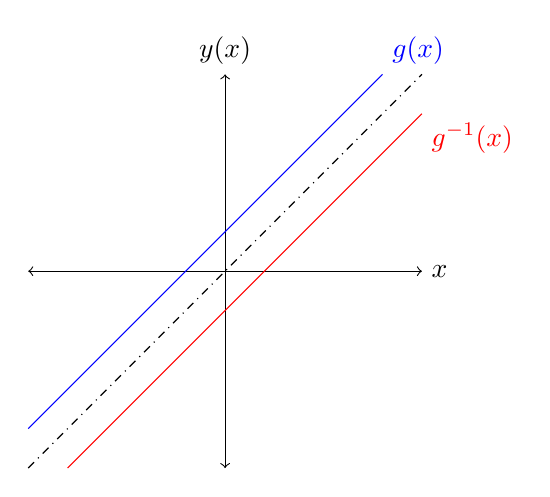
\begin{tikzpicture}[xscale=0.25,yscale=0.25]
      \draw[<->] (-10,0) -- (10,0) node[right] {$x$};
      \draw[<->] (0,-10) -- (0,10) node[above] {$y(x)$};
      \draw[scale=1,domain=-10:8,smooth,variable=\x,blue] plot ({\x},{\x+2}) node[above right] {$g(x)$};
      \draw[scale=1,domain=-10:10,smooth,variable=\x,black,dashdotted] plot ({\x},{\x});
      \draw[scale=1,domain=-8:10,smooth,variable=\x,red] plot ({\x},{\x-2}) node[below right] {$g^{-1}(x)$};
    \end{tikzpicture}
\end{figure}


One common way of thinking about this reflection property of inverses is that if you were to “fold” the graph diagonally along the line $y(x)=x$, functions that are inverses of each other would be folded onto each other.  

Another essential property of inverses $-$ arguably their defining property $-$ is that if you compose a function with its inverse (or vice versa) you end up with simply $x$.  That is to say: $$f^{-1}\left(f(x)\right)=f\left(f^{-1}(x)\right)=x.$$

This fact can act as a way to check to make sure two functions are inverses of each other.  Let’s use this in an example.

\begin{example}
Find the inverse, $f^{-1}(x)$, of $f(x)=2x-4$.  Then, on the same graph, sketch both $f(x)$ and $f^{-1}(x)$.  Finally, use the statement above to prove $f(x)$ and $f^{-1}(x)$ are inverse functions.
\end{example}
\begin{solution}
Starting off, let's solve for $f^{-1}(x)$.  We do this first by switching the independent and dependent variables.  This yields: $$x=2f^{-1}(x)-4.$$  Rearranging and solving for $f(x)$ gives $$2f^{-1}(x)=x+4 \implies f^{-1}(x)=\dfrac{1}{2}x+2.$$  Next, we will graph the two functions (along with $y(x)=x$) to visually confirm that $f(x)$ and $f^{-1}(x)$ are inverses using the reflection property stated above.  The graph is shown at the top of the next page due to spacing purposes.

Finally, let's check to make sure these functions are inverses.  We find both $f\left(f^{-1}(x)\right)$ and $f^{-1}\left(f(x)\right)$: \begin{align*}
    f\left(f^{-1}(x)\right)&= f\left(\dfrac{1}{2}x+2\right)=2\left(\dfrac{1}{2}x+2\right)-4=x+4-4=x \\
    f^{-1}\left(f(x)\right)&= f^{-1}\left(2x-4\right)=\dfrac{1}{2}\left(2x-4\right)+2=x-2+2=x
\end{align*}
Now that we've algebraically and graphically proven that these functions are inverses, we can confirm that we are indeed correct.  $\Box$
\end{solution}
This is all we need to cover for this section.  Let's discuss the final section of this chapter: piece-wise linear functions.

\begin{figure}[!h]
    \centering
    \begin{tikzpicture}[xscale=0.25,yscale=0.25]
      \draw[<->] (-10,0) -- (10,0) node[right] {$x$};
      \draw[<->] (0,-10) -- (0,10) node[above] {$y(x)$};
      \draw[scale=1,domain=-10:10,smooth,variable=\x,black,dashdotted] plot ({\x},{\x});
      \draw[scale=1,domain=-3:7,smooth,variable=\x,blue] plot ({\x},{2*\x-4}) node[above right] {$f(x)$};
      \draw[scale=1,domain=-10:10,smooth,variable=\x,red] plot ({\x},{\x/2+2}) node[below right] {$f^{-1}(x)$};
    \end{tikzpicture}
\end{figure}

\section{Piece-wise Linear Functions}
Finishing up the chapter we have understanding and graphing linear piece-wise functions.  While these functions aren't used incredibly often currently, they do have their applications in the real world and in higher-level mathematics.  Piece-wise functions in general can be thought of as a sort of Frankenstein’s monster: pieces of different functions mashed together into a single function.

In the case of linear piece-wise functions, we take two or more lines, chop them up, and put the pieces we want into a single function.  This idea can be best understood by graphing.
\begin{wrapfigure}{r}{4cm}
    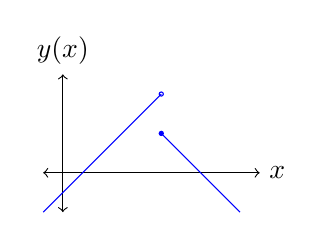
\begin{tikzpicture}[xscale=0.25,yscale=0.25]
      \draw[<->] (-1,0) -- (10,0) node[right] {$x$};
      \draw[<->] (0,-2) -- (0,5) node[above] {$y(x)$};
      \draw[scale=1,domain=-1:5,smooth,variable=\x,blue] plot ({\x},{\x-1});
      \draw[scale=1,domain=5:9,smooth,variable=\x,blue] plot ({\x},{7-\x});
      \filldraw[blue] (5,2) circle[radius=3pt];
      \draw[blue] (5,4) circle[radius=3pt];
    \end{tikzpicture}
\end{wrapfigure}
Here we can see the graph of the linear piece-wise function: $$y(x)=\begin{cases} x-1 & x < 5 \\ 7-x & x \geq 5 \end{cases}.$$
Something which piece-wise functions can do, something that you probably haven’t seen in any other function up until now, is that the function is not continuous; in layman’s terms, this means the graph has a “break” in it.  We can see that the graph appears to get closer to a $y$-value of $4$ as we move along the first line $f(x)=x-1$; all of a sudden however, once we reach $x=5$ the graph magically moves down to a $y$-value of $2$ onto the second line $g(x)=7-x$.  This idea of “continuity” (or, in this case, discontinuity) is extremely important later on in Calculus.

\begin{wrapfigure}{r}{2.5cm}
    \begin{tikzpicture}[xscale=0.5,yscale=0.5]
      \draw[<->] (-3,0) -- (3,0) node[right] {$x$};
      \draw[<->] (0,-1) -- (0,5) node[above] {$y(x)$};
      \draw[scale=1,domain=-3:0,smooth,variable=\x,blue] plot ({\x},{2-\x});
      \draw[scale=1,domain=0:3,smooth,variable=\x,blue] plot ({\x},{\x/2+1});
      \filldraw[blue] (0,2) circle[radius=3pt];
      \draw[blue] (0,1) circle[radius=3pt];
    \end{tikzpicture}
\end{wrapfigure}

Let’s take a look at another example with just $2$ lines so you can try graphing it.
\begin{example}
Graph the linear piece-wise function $$y(x)=\begin{cases} 2-x & x\in(-\infty,0] \\ \dfrac{1}{2}x+1 & x\in(0,\infty) \end{cases}.$$
\end{example}
\begin{solution}
Based on the interval to the right of the equations, we want to graph $f(x)=2-x$ for all $x$-values that are negative (and 0); likewise, we need to graph the second function $g(x)=\dfrac{1}{2}x+1$ for all positive values of $x$.  This leaves us with the final graph on the right.
\end{solution}

\begin{wrapfigure}{r}{2.5cm}
    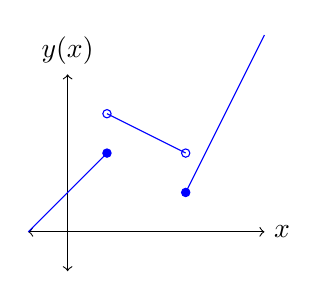
\begin{tikzpicture}[xscale=0.5,yscale=0.5]
      \draw[<->] (-1,0) -- (5,0) node[right] {$x$};
      \draw[<->] (0,-1) -- (0,4) node[above] {$y(x)$};
      \draw[scale=1,domain=-1:1,smooth,variable=\x,blue] plot ({\x},{\x+1});
      \draw[scale=1,domain=1:3,smooth,variable=\x,blue] plot ({\x},{-\x/2+7/2});
      \draw[scale=1,domain=3:5,smooth,variable=\x,blue] plot ({\x},{2*\x-5});
      \filldraw[blue] (1,2) circle[radius=3pt];
      \filldraw[blue] (3,1) circle[radius=3pt];
      \draw[blue] (1,3) circle[radius=3pt];
      \draw[blue] (3,2) circle[radius=3pt];
    \end{tikzpicture}
\end{wrapfigure}

Let’s do one more example to finish the chapter off, this time with three segments.  Remember that three segments works just the same as two.  This example will also have you use the graph to deduce the function; follow the same process for this as you would any other function.  Simply keep domain restrictions in mind.
\begin{example}
Write down the piece-wise function corresponding to the following graph.
\end{example}
\begin{solution}
Let’s go from left to right, figuring out the different segments we have in the graph.  On the left we have a line with slope $1$ and $y$-intercept of $1$; this segment goes from $-\infty$ to $1$.  This gives $$y_1(x)=mx+b=x+1 \hspace{0.25in} x\in(-\infty,1].$$
For the middle section, we see the line has a slope $-\dfrac{1}{2}$ but no $y$-intercept is shown; therefore, we must use the point slope formula (we will use the point $(1,3)$ from the segment): $$y_2(x)=y_0+m(x-x_0)=3-\dfrac{1}{2}(x-1)=-\dfrac{1}{2}+\dfrac{7}{2} \hspace{0.25in} x\in(1,3).$$
For the final right-most segment, we see it has a slope of $2$, however once again no $y$-intercept is shown so we must use the point-slope formula again; this segment stretches from $3$ to $\infty$.  $$y_3(x)=y_0+m(x-x_0)=1+2(x-3)=2x-5 \hspace{0.25in} x\in[3,\infty).$$
Putting this all together gives us our final function: $$y(x)=\begin{cases} y_1(x) \\ y_2(x) \\ y_3(x) \end{cases} = \begin{cases} x+1 & x \leq 1 \\ -\dfrac{1}{2}x+\dfrac{7}{2} & 1<x<3 \\ 2x-5 & x \geq 3 \end{cases}.$$ $\Box$
\end{solution}
This is everything we needed to cover in this chapter.  Again, it was very short.  Ensure that you have complete mastery of the skills used here so that we can continue to refer to them throughout the text.  This chapter also does not have a challenge set; the problems don't get overly difficult.
\begin{reviewset}
\item For each part, graph $f(x)$ and $f^{-1}(x)$ without computing $f^{-1}(x)$.  \newline 
(a) $f(x)=4$ \hspace{60mm} (b) $f(x)=2x$ \newline 
(c) $f(x)=\dfrac{1-7x}{3}$ \hspace{50mm} (d) $f(x)=\dfrac{1}{2}x-1$ \vspace{3mm}

\item What value of $x$ satisfies $x-\dfrac{3}{4}=\dfrac{5}{12}-\dfrac{1}{3}$? \vspace{3mm}

\item Graph $y(x)=\begin{cases} 2x-3 & -\infty < x \leq 2 \\ 1-\dfrac{7}{2}x & 2 < x \leq 3 \\ 4 & x > 3 \end{cases}$.  \vspace{3mm}

\item Determine the range of the following functions over the given domain.  \newline
(a) $f(x)=4$ \hspace{60mm} (b) $f(x)=7x-2$ \newline 
(c) $f(x)=\dfrac{3}{2}-\dfrac{4}{3}x$ \hspace{49mm} (d) $f(x)=\dfrac{5x-4}{16}$ \vspace{3mm}

\item Solve: $x-\dfrac{1-\frac{3x}{2}}{4}=\dfrac{2-\frac{x}{4}}{3}-\dfrac{11}{12}$ for $x$.  \vspace{3mm}

\item Solve the following word problems.  \newline 
(a) A number is equal to 7 times itself minus 18.  Which is the number? \newline 
(b) A number is equal to 4 times this number less 75.  What is the number? \newline 
(c) Two times a number, decreased by 12 equals three times the number, decreased by 15.  Which is the number? \newline 
(d) Twice a number equals 5 times the same number plus 18.  Which is the number? \vspace{3mm}

\item Let $f(x)=\dfrac{4x-5}{12}$.  Determine the smallest integer $n$ such that $f(n)>0$.  \vspace{2mm}.

\item Without computing $f^{-1}(x)$, determine the intersection point of $f(x)=\dfrac{1}{3}x-3$ and $f^{-1}(x)$.  \vspace{3mm}

\item For the following functions, compute $f^{-1}(x)$.  Note that $a_1,a_2\in\mathbb{R}$ and $a_1,a_2\neq 0$.  \newline 
(a) $f(x)=x-1$ \hspace{50mm} (b) $f(x)=\dfrac{2x-1}{3}$\newline 
(c) $f(x)=\dfrac{5}{6}x-\dfrac{4}{5}$\hspace{47mm} (d) $f(x)=a_1x+a_2$ \vspace{3mm}

\item Suppose $f(x)=kx+k$ where $k\in\mathbb{R}$.  Find all values of $k$ such that $f(x)\cdot f^{-1}(x)=x^2-3x-4$.  \vspace{3mm}

\item An ideal spring is defined such that the force ($F$, in Newtons) exerted is proportional to the compression distance ($\Delta x$, in metres).  A physics teacher wants to test this constant of proportionality, called the spring constant ($k$, in Newtons per meter).  He attaches a spring to the ceiling with two different weights.  The $1.5N$ block stretches the spring $0.25m$ and the $2.4N$ block stretches the spring $0.4m$.  Determine the value of $k$, the spring constant.  \vspace{3mm}

\item Let $f(x)=\begin{cases} 1-2x & x \leq k \\ \dfrac{3}{2}x-5 & x > k \end{cases}$.  Determine the value of $k$ that makes $f(x)$ continuous.  \vspace{3mm}

\item Let $f(x)$ be a linear function such that $f(6)-f(2)=12$.  Compute $f(12)-f(2)$.  [$\star$] \vspace{1mm}

\item Determine the area bound by the $x$-axis, the $y$-axis, and $y=1-2x$.  [$\star$]
\end{reviewset}
\end{document}